\chapter{Methoden}   \label{ch_3}
In diesem Kapitel wird die empirische Bearbeitung der Hypothesen dargestellt. Zunächst wird die erhobene Stichprobe beschrieben, gefolgt von der Erläuterung der Erhebungsmethode, Stichprobenauswahl und das Erhebungsdesign. Darauf folgend wird auf die Operationalisierung der Konstrukte eingegangen. In folgendem Zuge wird die Untersuchungsdurchführung konkretisiert und abschließend wird auf die Auswertungsmethode eingegangen.

\section{Stichprobenbeschreibung} \label{sec_3.1}
Von den 578 Probanden, die den Onlinebefragung ausgefüllt hatten, mussten 145 entfernt werden, da sie den Fragebogen nicht vollständig beantwortet hatten. Aufgrund ungültiger Werte und beleidigender Kommentare musste eine weitere Person entfernt werden. Somit nahmen am Onlinefragbogen eine Stichprobe von $N~=~432$ Probanden teil. \begin{figure}[htb]
    \centering
        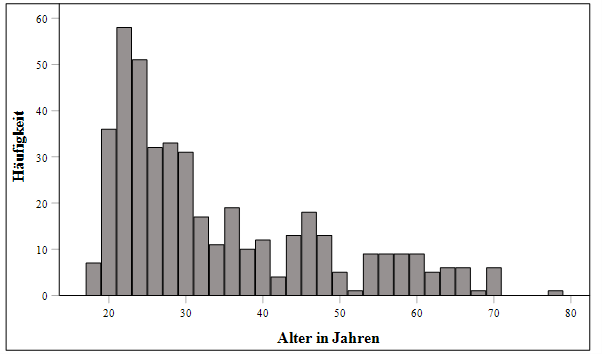
\includegraphics[width=0.8\linewidth]{Histogramm - Altersverteilung.png}
        \caption[Histogramm Altersverteilung]{Histogramm für die Altersverteilung.}
        \label{Histogramm Altersverteilung}
\end{figure}


Mit $n~=~305$ (70.60\%) bilden weibliche Teilnehmer den größten Teil der Gesamtstichprobe ab. Männliche Teilnehmer betrugen 28.9\% ($n~=~125$) der Befragten. Des Weiteren gaben 0.5\% ($n~=~2$) der Probanden an ein diverses Geschlecht zu haben. Das Durchschnittsalter der Teilnehmer lag bei $M~=~33.52$ Jahren ($SD~=~13.67$). Eine grafische Darstellung der Altersverteilung ist in Abbildung~\ref{Histogramm Altersverteilung} zu sehen. An ihr lässt sich ablesen, dass der jüngste Teilnehmer 18 Jahre alt war, der älteste betrug ein Alter von 77 Jahren. Es handelt sich dabei um eine unimodale und rechtsschiefe Verteilung. 
 % Modus 21 Jahre, da ein großer Teil der Probanden Studenten waren.


\section{Untersuchungsdesign}  \label{sec_3.2}
Die vorliegende Studie ist Teil eines größeren Forschungsprojektes, das weitere vier Arbeiten, mit ihren jeweiligen Schwerpunkten, beinhaltet. Jede dieser Arbeiten beschäftigte sich mit den Themen der häuslichen Gewalt und das der Gewaltmythen. Das Gesamtprojekt wurde am 02.06.2022 präregistriert. Bevor der Fragebogen zur Erhebung freigegeben werden konnte, lief er einen Pretest vom 30.05.2022 bis 02.06.2022 durch. So konnten mögliche Fehler und Probleme behoben werden, um eine gute Durchführung für die Teilnehmer zu gewährleisten. 

Vorraussetzung für die Teilhabe an der Umfrage waren ein internetfähiges Endgerät, die Erreichte Volljährigkeit und eine ausreichende Beherrschung der deutschen Sprache. 

Für die Datengeneration wurde ein Onlinefragbogen erstellt, da dadurch eine weitreichendere und ökonomischere Erhebung gewährleistet werden konnte. Auf diese weise konnnten der Interview- und der Versuchsleitereffekt vermieden werden. Der Zugangslink wurde primär über die sozialen Netzwerke der Projektleiterinnen verschickt der sich nach dem Primzip des Schneeballeffekts verbreitete. Es handelt sich dabei um ein randomisiertes teilexperimentelles Verfahren mit einer anfallenden Stichprobe. Das Verfahren ist teilexperimentel, da die Variablen in den Fallvignetten manipuliert wurden, die Variablen der standatisierten Fragebögen jedoch nicht.

Bezüglich der Erhebungsmethode und -Design handelt es sich bei dieser Arbeit um eine quantitative Querschnittstudie, auf der Basis eines einzigen Messzeitpunktes.

Für die Ergebng der Daten wurde neben den Vignetten eine deutsche Übersetzung des Domestic Violence Myth Acceptance Scala (DVMAS) nach \textcite{Peters2003}. Bei zügkunfiten Nennungen des DVMAS wird stehts die deutsche Übersetzung referenziert. Für die Erhebung der Aggression wurde der Deutsche Aggressionsfragebogen von \textcite{Aggressionsfragebogen} verwendet.


\section{Operationalisierung der Konstrukte}    \label{sec_3.3}
Damit die Teilnehmer unvoreingenommen die, der Wahrheit ähnelten, fiktiven Fallvignetten bewerten konnten, begann der Fragebogen mit zwei zufällig zugeodneten Vignetten, die psychische oder sexualisierte Gewalt behandelten. Darauf folgte die deutsche Version der Skala zur Erfassung der Akzeptanz von Gewaltmythen. Im Anschluss befand sich eine umfangreiche Testbatterie mit vier Skalen um physische wie verbale Aggression, den Ärger und das Misstrauen zu messen. Abschließend wurden die soziodemografischen Daten wie Alter, Geschlecht, kultureller Hintergrund, Bildungsstand, berufliche Situation und das Einkommen erfragt.

Mithilfe der Fallvignetten zur häuslichen Gewalt wurde die Verantwortungszuschreibung erhoben. Insgesamt wurden 16 unterschiedliche Vignetten generiert, um vier verschiedene Variablen messen zu können. Bei diesen Variablen handelte es sich umd die Gewaltart (psychisch oder sexualisiert), das Geschlecht (männlich oder weiblich), den sozioökonomischen Status (hoch oder niedrig) und um den kulturellen Hintergrund (deutsch oder arabisch). Über einen Schiberegler konnten die Probanden die relative Verantwortung von Opfer und Täter bewerten. Die Codierung verlief vom kleinstmöglichen Punktewert auf der linken Seit bis zum größtmöglichen Punktewert auf der rechten Seite (Codierung 1-101). Jeder Proband bekam sowohl eine Vignetter sexualisierter Gewalt wir einer psychischer. Die Ausprägungen der anderen drei Variablen wurden randomisiert zugeteilt.
Ein Beispiel für eine psychische Gewaltvignette mit arabischem Hintergrund, einem weiblichen Opfer und einem niedrigeren sozioökonomischen Status des Opfers sah wie folgt aus: \textit{Mustafa arbeitet als Arzt im öffentlichen Krankenhaus. Seine Frau Fatima darf ihm zuhause nicht widersprechen. Sogar in der Öffentlichkeit verbietet Mustafa ihr häufig den Mund. Dadurch sinkt das Selbstwertgefühl von Fatima so weit, dass sie viel im Bett liegt und kaum noch Freude an Freizeitaktivitäten und ihrem 450$-$Ehro$-$Job als Kassiererin hat.} 
Eine psychische Fallvignette konnte wie folgt aussehen: %Vignette.

Die Akzeptanz von häuslichen Gewaltmythen wurden mithilfe der deutschen Übersetzung des englischen Domestic Violence Myth Acceptance Scale (DVMAS) \parencite{Peters2003} unternommen. Bis auf das letzte Item sind alle übrigen 17 Items als Aussagen vormuliert und wurden mithilfe einer siebenstufigen Skala, von 1 = \enquote{Stimme überhaupt nicht zu} bis 7 = \enquote{Stimme völlig zu}, beantwortet. Ein solches Item war wie folgt: \textit{Einen Mann eifersüchtig zu machen, ist wie eine Provokation zur Gewalt.}
Für die deutsche Übersetzung des DVMAS liegt bislang noch keine Validierung vor. Da es hierbei um eine Sinngemäße Übersetzung handelt wird die Reliabilität und Validität des originalen DVMAS herangezogen. Die Reliabilität von Cronbachs-\textalpha~=~.88 liegt in einem sehr gute Bereich. Des Weiteren liegt auch eine gute Validität vor, zumal der DVMAS signifikante Korrelationen mit den folgenden vier theoretisch ähnelnden Skalen aufweist: Attitude Towards Women, Rape Myth acceptance scale, Sex Role Stereotypes und Attitude Towards Wife Abuse \parencite{DVMAS_Peters}.

Das letzte erhobene Konstrukt Aggression wurde mithilfe des Deutschen Aggressionsfragebogens erfasst. Dieser umfasst 29 Items verteilt auf den folgenden vier Subskalen: physische Aggression, verbale Aggression, Ärger und Misstrauen. Die als Aussage formulierten Items wurden anhand einer vier-stufigen Likertskala von 1 = \enquote{trifft nich zu} bis 4 = \enquote{trifft voll zu} beantwortet. Ein solches Item war wie folgt: \textit{Manchmal verzehrt mich Eifersucht.} Dies ein Beispiel aus der Aggression-Subskala Misstrauen. Die Validität des Fragebogens wurde durch die signifikante Korrelationen mit Aggressivität, generalisierter Selbstwert, Ärger, Ärgerkontrolle und Neurotizismus festgestellt. Die Reliabilität variiert zwischen \textalpha~=~.62 und \textalpha~=~.82 (Cronbachs-\textalpha der Subskalen) und weißt eine Retestreliabilität von Cronbachs-\textalpha~=~.73\parencite{Aggressionsfragebogen}.

Die Reliabilität ist aufgrund des standatisierten Fragebogens gegeben. Es kann auch von einer gegebenen Objektivität ausgegangen werden, weil ohne einen Versuchsleiter die Probanden den Fragebogen eigenständig durchgeführten mussten. Aufgrund der Relevanz dieser Befragung ist sie valide.



\section{Untersuchungsdurchführung}   \label{sec_3.4}
Über den Zeitraum vom 04.06.2022 bis 27.06.2022 erstreckte sich die Datenerhebung. Der über SoSci-Survey erstellte Fragebogen wurde primär über den Messenger-Dienst WhatsApp, aber auch über Instagram, Facebook, Signal, Telegram und das Alumniportal Deutschland verbreitet, mit der Bitte der Verbreitung, um eine möglichst große Stichprobe zu erreichen. Die Mindeststichprobengröße von 395 wurde mithilfe des kostenlosen Tools G*Power ermittelt. %G*Power (https://bjoernwalther.com/eine-kurze-einfuehrung-in-gpower/)


Im Einführungstext, zu Beginn der Befragung, wurden Auskünfte über die 15 minütige Bearbeitungszeit, wie auch die garantierte Anonymität der Probanden aufgeklärt. In der Werbung und im Einführungstext wurden Begriffe häusliche Gealt, Gewaltmythen und Gewalt bewust vermieden, um eine Beeinflussung auf die Anstehende Verantwortungszuschreibung zu vermeiden. Die Teilnehmer wurden zudem darauf hingewiesen, dass die Teilnahme der Befragung freiwillige ist. Bevor auf die nächste Seite weitergeklickt werden konnte, wurde mithilfe einer zu beantworteten Frage sichergestellt, dass die Person den Einleitungstext verstanden hat und mit der Befragung einverstanden ist. Auf der anschließenden Seite folgte die Aufgabenerklärung für die Fallvignetten, wie eine kleine Aufklärung diesbezüglich. Jeweils nach jeder dargebotener Vignette folgten vier Fragen, zur überprüfung der Manipulation. Durch die nachfolgende Frage wurde das Erkennen der Gewaltart überprüft: \textit{Ging es um sexualisierte Gewalt?}. Die anschließende Frage überprüfte das Geschlecht des Opfers: \textit{Was das Opfer eine Frau?}. Anschließend folgte die Nachfrage nach dem sozioökonomischen Status: \textit{War die finanzielle Situation des Opfers schlechter als die finanzielle Situation des Täters?}. Zum Schluss wurde die vierte und letzte Variable, der kultuerlle Hintergrund, überprüft: \textit{Hatten die Personen deutsche Namen?}. Anschließend folgten die deutsche Übersetzung des DVMAS und der Deutsche Aggressionsfragebogen. Zum Schluss wurden die Probanden gebeten einige kurze Angaben zu ihrer Person zu geben, woraufhin eine letzte Nachfrage der gewissenhaften Durchführung folgte. Die Probanden konnten noch eine freiwillige Vermutung der zu untersuchten Themen in ein Feld eintragen. Dies bietete eine weitere Möglichkeit zu überprüfen, ob die Teilnehmer aufmerksam den Fragebogen bearbeitet hatten. Damit endete der für die Forschenden wichtige Teil der Befragung. Auf einer daran anschließenden Seite wurden Informationen und Kontaktdaten für Betroffene von häuslicher Gewalt gewährleistet. 

Mit Abschließen der befragung wurden die Probanden, die über das SONA-System kamen wieder dorthin zurückgeführt und ihnen wurden 0.25 Versuchspersonenstunden angerechnet.

Potenzielle Störvariablen konnten während der Untersuchungsdurchführung nicht kontrolliert werden. Anhand der Onlinebefragung lag die Entscheidung, zu welchem Zeitpunkt, an welchem Ort und unter welchen Bedingungen die Befragung bearbeitet wurde, bei den Teilnehmern selbst.


\section{Auswertungsmethode}    \label{sec_3.5}
Der erhobene Datensatz wurde mithilfe der Statistik- und Analysesoftware SPSS berechnet. Bevor die Hypothesen jedoch berechnet werden konnten, musste der Datensatz bereinigt werden. So, wie die Fallvignetten im Fragebogen konzipiert waren, musste der Datensatz verdoppelt werden, damit mit den Daten der Vignetten gerechnet werden konnte. 

Anschließend konnten die Daten ausgewertet werden, beginnend mit den deskriptiven Kennzahlen der drei Konstrukte. Anhand der Lageparameter, der Maße der Streuung und der Verteilung konnten die demographischen Daten der Stichprobe ausgewertet werden.

Damit die Fallvignetten wie auch der Aggressionsfragebogen für die Berechnungen genutzt werden konnten, mussten jeweils einige Items umgepolt werden. Damit bei den Vignetten den betroffenen Person stets der Zahlenwert 101 (Schieberegler rechts) zugeordnet wird, wurden jeweils bei den psychischen und sexualisierten Vignetten drei Fälle umkodiert. Ferner beinhalteten die Vignetten weitere Variablen, die für die Auswertung bei dieser Arbeit, wie auch bei den Auswertungen der weiteren Projektmitglieder wichtig waren. Für die individuelle Verwendung dieser, wurden sie aus den entsprechenden Fallvignetten extrahiert und jeweils zu einer separaten dummy-kodierten Variable dichotomisiert. Beim Aggressionsfragebogen wurden Item 14 \enquote{Ich bin eine ausgeglichene Person.} und Item 22 \enquote{Ich kann mir keinen Grund vorstellen, weshalb ich jemals eine andere Person schlagen würde.} umgepolt.

Die in Kapitel ~\ref{sec_3.4} bereits erwähnten Manipulationschecks wurden mithilfe des Chi$^2$-Tests berechnet.

Die erste Hypothese (H1) wurde mit der Spearman$-$Rang$-$Korrelation berechnet. Die H1 untersuchte eine positive Korrelationen zwischen dem metrischen Aggressionsscore und der metrischen Verantwortungszuschreibung auf das Opfer. Neben der mindestens ordinalen Skalierung der Variablen, setzt die Spearman$-$Rang$-$Korrelation eine paarweise Beobachtung voraus.  

Für die zweite Hypothese (H2) wurde eine Pearson$-$Produkt$-$Moment$-$Korrelationen gerechnet. Die Korrelationsrechnung der H2 diente der Überprüfung der angenommenen positiven Korrelation des metrischen Aggressionsscores mit der metrischen Akzeptanz von Gewaltmythen. Voraussetzungen für eine Pearson$-$Produkt$-$Moment$-$Korrelation sind die Intervallskalierung oder Dichotomie beider Variablen, eine bestehende Linearität, die Abwesenheit von Ausreißern, sowie die Endlichkeit der Varianz beziehungsweise. Kovarianz.

Bei der dritten Hypothese (H3) handelte es sich um eine Moderationsanalyse, die mithilfe des Plug-in PROCESS berechnet wurde. Untersucht wurde bei dieser Hypothese ob das Geschlecht den Zusammenhang zwischen Akzeptanz von Gewaltmythen und Aggression moderiert. Die allgemeinen Vorraussetzung für diesen Test sind die Linearität und der Stichprobenumfang. Des Weiteren gibt es spezifische Voraussetzungen. Eine gegebene Homoskedastizität, Normalverteilung des Fehlers, keine Autokorrelation und keine Multikolinearität müssen gegeben sein.